\chapter{Q12}
\emph{Q12: Explain how ESRT and CODA work? What are the difference between ESRT
and CODA?}

\section{ESRT}
\emph{Event-to-Sink Reliable Transport protocol}

If $r_i > R$ then the event is reliably detected; else appropriate actions must
be taken to achieve $R$.

\subsection{Source}
\begin{description}
	\item Send data with reporting frequency $f$ 
	\item Monitor buffer level and notify congestion to the sink.
\end{description}

\subsection{Sink}

\begin{description}
	\item Measures the observed event reliability $r_i$ at interval $i$
	\item Normalized Reliability $n_i = \frac{r_i}{R}$
	\item Performs congestion decision based on the feedback from the sensor
		nodes
	\item Broadcasts the new reporting rate to all sensor nodes
\end{description}

\begin{figure}[h]
	\centering
	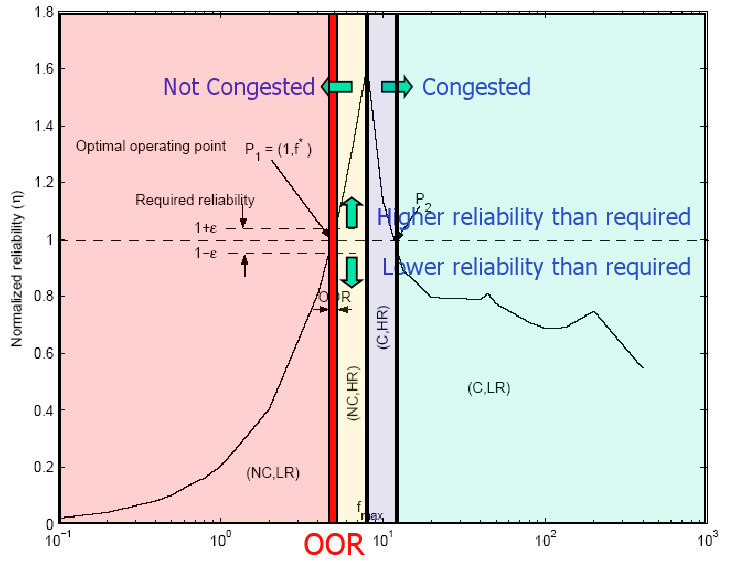
\includegraphics[scale=0.4]{img/CongestionDetection-ESRT.png}
\end{figure}

\section{CODA} 
\emph{Congestion Detection and Avoidance}

Energy efficient congestion control.

Three mechanisms are involved:
\subsection{Congestion detection}

\subsubsection{Indication of congestion}
\begin{description} 
	\item nearly overflowing queue
	\item measured channel load higher the optimum utilization
\end{description}

\subsubsection{CSMA}
When using CSMA empty buffer indicates that congestion is mitigated.


\subsection{Open-loop hop-by-hop backpressure}

\begin{description}
	\item Do local congestion detection at each node with low cost
	\item Congestion is detected $\rightarrow$ the node broadcasts suppression
		message to upstream neighbors
	\item Make local adjustments to prevent propagating the congestion
		downsteam
\end{description}

Receiving backpressure signals:
\begin{description}
	\item Reduce sending rate or drop packets
	\item Choose which packets to drop
	\item Decide whether or not to propagate the backpressure signal
\end{description}

\subsection{Closed-loop multi-source regulation}

When the source event rate $r$ is less than some fraction $n$ of
the maximum theoretical throughput of the channel $S_{MAX}$, the
source regulate itself.

When $r \geq nS_{MAX}$, a source is more likely to contribute to congestion and
closed-loop control is triggered (i.e. source triggers sink regulation)

\begin{description}
	\item Source sets a regulate bit in the data packets
	\item If the sink receives a packet with regulate bit set, the sink has to
		send ACKs to regulate sources associated with a particular event. (e.g.
		1 ACK per 100 data packets)
	\item If the source recive ACK, continue at $r$
	\item If congestion $\rightarrow$ ACK is lost and source lowers $r$
\end{description}


